% Copyright (c) 2022 by Lars Spreng
% This work is licensed under the Creative Commons Attribution 4.0 International License. 
% To view a copy of this license, visit http://creativecommons.org/licenses/by/4.0/ or send a letter to Creative Commons, PO Box 1866, Mountain View, CA 94042, USA.

%~~~~~~~~~~~~~~~~~~~~~~~~~~~~~~~~~~~~~~~~~~~~~~~~~~~~~~~~~~~~~~~~~~~~~~~~~~~~~~
% You can add your packages and commands to the loadslides.tex file. 
% The files in the folder "styles" can be modified to change the layout and design of your slides.
% I have included examples on how to use the template below. 
% Some of it these examples are taken from the Metropolis template.
%~~~~~~~~~~~~~~~~~~~~~~~~~~~~~~~~~~~~~~~~~~~~~~~~~~~~~~~~~~~~~~~~~~~~~~~~~~~~~~


\documentclass[18pt,notheorems,hyperref={pdfauthor=whatever}]{beamer}


% Copyright (c) 2022 by Lars Spreng
% This work is licensed under the Creative Commons Attribution 4.0 International License. 
% To view a copy of this license, visit http://creativecommons.org/licenses/by/4.0/ or send a letter to Creative Commons, PO Box 1866, Mountain View, CA 94042, USA.

%~~~~~~~~~~~~~~~~~~~~~~~~~~~~~~~~~~~~~~~~~~~~~~~~~~~~~~~~~~~~~~~~~~~~~~~~~~~~~~
% Add your packages and commands to this file
%~~~~~~~~~~~~~~~~~~~~~~~~~~~~~~~~~~~~~~~~~~~~~~~~~~~~~~~~~~~~~~~~~~~~~~~~~~~~~~

%~~~~~~~~~~~~~~~~~~~~~~~~~~~~~~~~~~~~~~~~~~~~~~~~~~~~~~~~~~~~~~~~~~~~~~~~~~~~~~
\RequirePackage{palatino}
\RequirePackage[utf8]{inputenc}
\RequirePackage[T1]{fontenc}

\usefonttheme{serif}
\usepackage{alphabeta}
\usepackage{styles/elegantmacros}
\usefolder{styles}
\usetheme[style=blue]{elegant}

\newcommand{\makepart}[1]{ % For convenience
\part{#1} \frame{\partpage}
}

%~~~~~~~~~~~~~~~~~~~~~~~~~~~~~~~~~~~~~~~~~~~~~~~~~~~~~~~~~~~~~~~~~~~~~~~~~~~~~~

%~~~~~~~~~~~~~~~~~~~~~~~~~~~~~~~~~~~~~~~~~~~~~~~~~~~~~~~~~~~~~~~~~~~~~~~~~~~~~~
% Figures
\RequirePackage{booktabs}
\RequirePackage{colortbl}
\RequirePackage{ragged2e}
\RequirePackage{schemabloc}
%\RequirePackage{natbib}
\RequirePackage{caption}
\RequirePackage{subcaption}
\RequirePackage{tabularx}
\RequirePackage{array}
\RequirePackage{multirow}
\usepackage[
  style=authoryear, 
]{biblatex}
\addbibresource{references.bib}
\newcolumntype{Y}{>{\centering\arraybackslash}X}

%~~~~~~~~~~~~~~~~~~~~~~~~~~~~~~~~~~~~~~~~~~~~~~~~~~~~~~~~~~~~~~~~~~~~~~~~~~~~~~

%~~~~~~~~~~~~~~~~~~~~~~~~~~~~~~~~~~~~~~~~~~~~~~~~~~~~~~~~~~~~~~~~~~~~~~~~~~~~~~
% Figures
\RequirePackage{wrapfig}
\RequirePackage{pgfplots}
\RequirePackage{graphicx}
\RequirePackage{adjustbox}
\RequirePackage{environ}
\pgfplotsset{compat=1.18}

\makeatletter
\newsavebox{\measure@tikzpicture}
\NewEnviron{scaletikzpicturetowidth}[1]{%
  \def\tikz@width{#1}%
  \def\tikzscale{1}\begin{lrbox}{\measure@tikzpicture}%
  \BODY
  \end{lrbox}%
  \pgfmathparse{#1/\wd\measure@tikzpicture}%
  \edef\tikzscale{\pgfmathresult}%
  \BODY
}
\makeatother
%~~~~~~~~~~~~~~~~~~~~~~~~~~~~~~~~~~~~~~~~~~~~~~~~~~~~~~~~~~~~~~~~~~~~~~~~~~~~~~

%~~~~~~~~~~~~~~~~~~~~~~~~~~~~~~~~~~~~~~~~~~~~~~~~~~~~~~~~~~~~~~~~~~~~~~~~~~~~~~
% Maths 
\RequirePackage{textcomp}
\RequirePackage{amsmath} 
\RequirePackage{amsthm}
\RequirePackage{mathtools}
%\RequirePackage{bbm}
%\RequirePackage{algorithm}
%\RequirePackage[osf,sc]{mathpazo}
%\RequirePackage{pifont}
%\newcommand{\xmark}{\ding{55}}%
%\numberwithin{equation}{section}
\DeclareMathOperator*{\argmax}{arg\,max}
\DeclareMathOperator*{\argmin}{arg\,min}

\setbeamertemplate{theorems}[numbered] % to number

\theoremstyle{definition}
\newtheorem{fact}{Fact}[section]
\newtheorem{examp}{Example}[section]

\theoremstyle{plain}
\newtheorem{definition}{Definition}[section]
\newtheorem{proposition}{Proposition}
\newtheorem{theorem}{Theorem}
\newtheorem{assumption}{Assumption}

\providecommand{\H}{\mathscr{H}}      
\providecommand{\E}{\mathbb{E}}
\makeatletter
\def\munderbar#1{\underline{\sbox\tw@{$#1$}\dp\tw@\z@\box\tw@}}
\makeatother

%~~~~~~~~~~~~~~~~~~~~~~~~~~~~~~~~~~~~~~~~~~~~~~~~~~~~~~~~~~~~~~~~~~~~~~~~~~~~~~
 % Loads packages and some defined commands

\title[
% Text entered here will appear in the bottom middle
]{Το Πείραμα STAR}

%\subtitle{Θωμόπουλος Σπύρος}

\author[
% Text entered here will appear in the bottom left corner
]{
    Θωμόπουλος Σπύρος 
}

\institute{
Τεχνολογία Ανιχνευτικών \& Επιταχυντικών Διατάξεων\\
    Σ.Ε.Μ.Φ.Ε.
}


\date{\today}

\begin{document}

% Generate title page

{
\usebackgroundtemplate{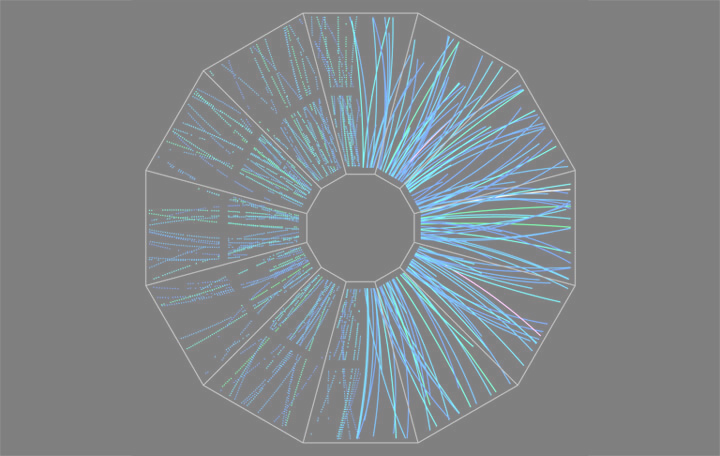
\includegraphics[height=13cm,width=20cm]{images/1st_op.png}}% make sure to reduce the opacity of the BG before uploading it

\begin{frame} 
    \maketitle
\end{frame}
}

\addtocounter{framenumber}{-1}

% You can declare different parts as a parentof sections
%\begin{frame}{Part I: Demo Presentation Part}
%    \tableofcontents[part=1]
%\end{frame}
%\begin{frame}{Part II: Demo Presentation Part 2}
%    \tableofcontents[part=2]
%\end{frame}
%
%-----------------------------------------------------------------------
%
%       STAR  Experiment 
%
%------------------------------------------------------------------------
%
% 1st STAR figure

\begin{frame}{Τί είναι το STAR(Solenoid TARcker);}
    \begin{figure}
        \centering
        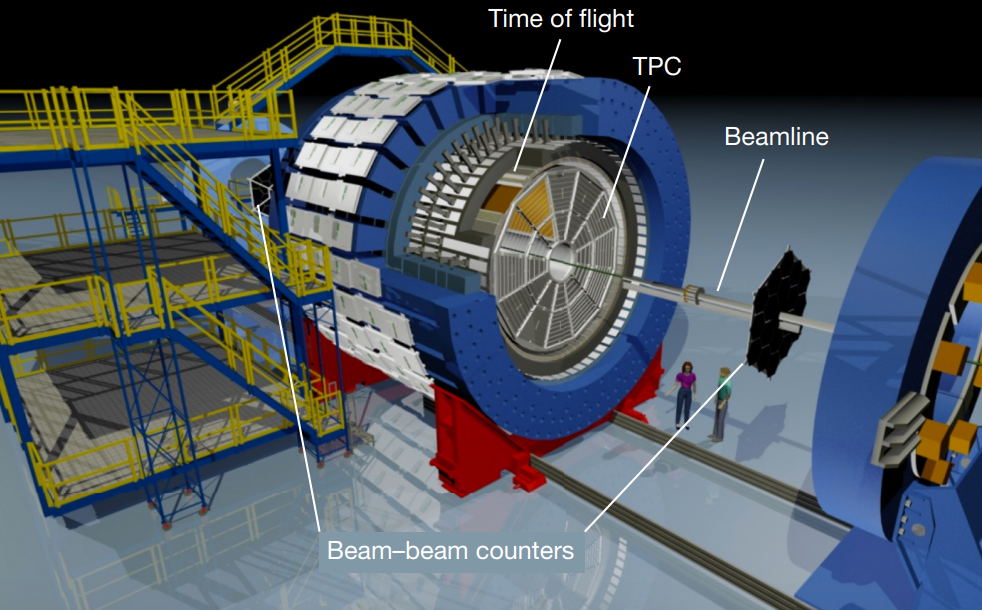
\includegraphics[scale=0.6]{images/STAR.png}
        %\caption{Caption}
        %\label{fig:my_label}
    \end{figure}
\end{frame}


% First     questions 
%\begin{frame}
%    \begin{itemize}
%        %\item[$\star$] {\Large }
%%        \item[$\star$] {\Large Τί ανιχνεύει; }                          \pause\vspace{+0.5cm}
 %       \item[$\star$] {\Large Από πού προέρχονται αυτά που ανιχνεύει; }\pause\vspace{+0.5cm}
 %       \item[$\star$] {\Large Πώς ανιχνεύει; }                         \pause\vspace{+0.5cm}
 %       \item[$\star$] {\Large Ποιοί είναι οι στόχοι του; }             \pause\vspace{+0.5cm}
 %   \end{itemize}
%\end{frame}


\begin{frame}{Επιτάχυνση}
    \begin{figure}[h!]
        \centering
        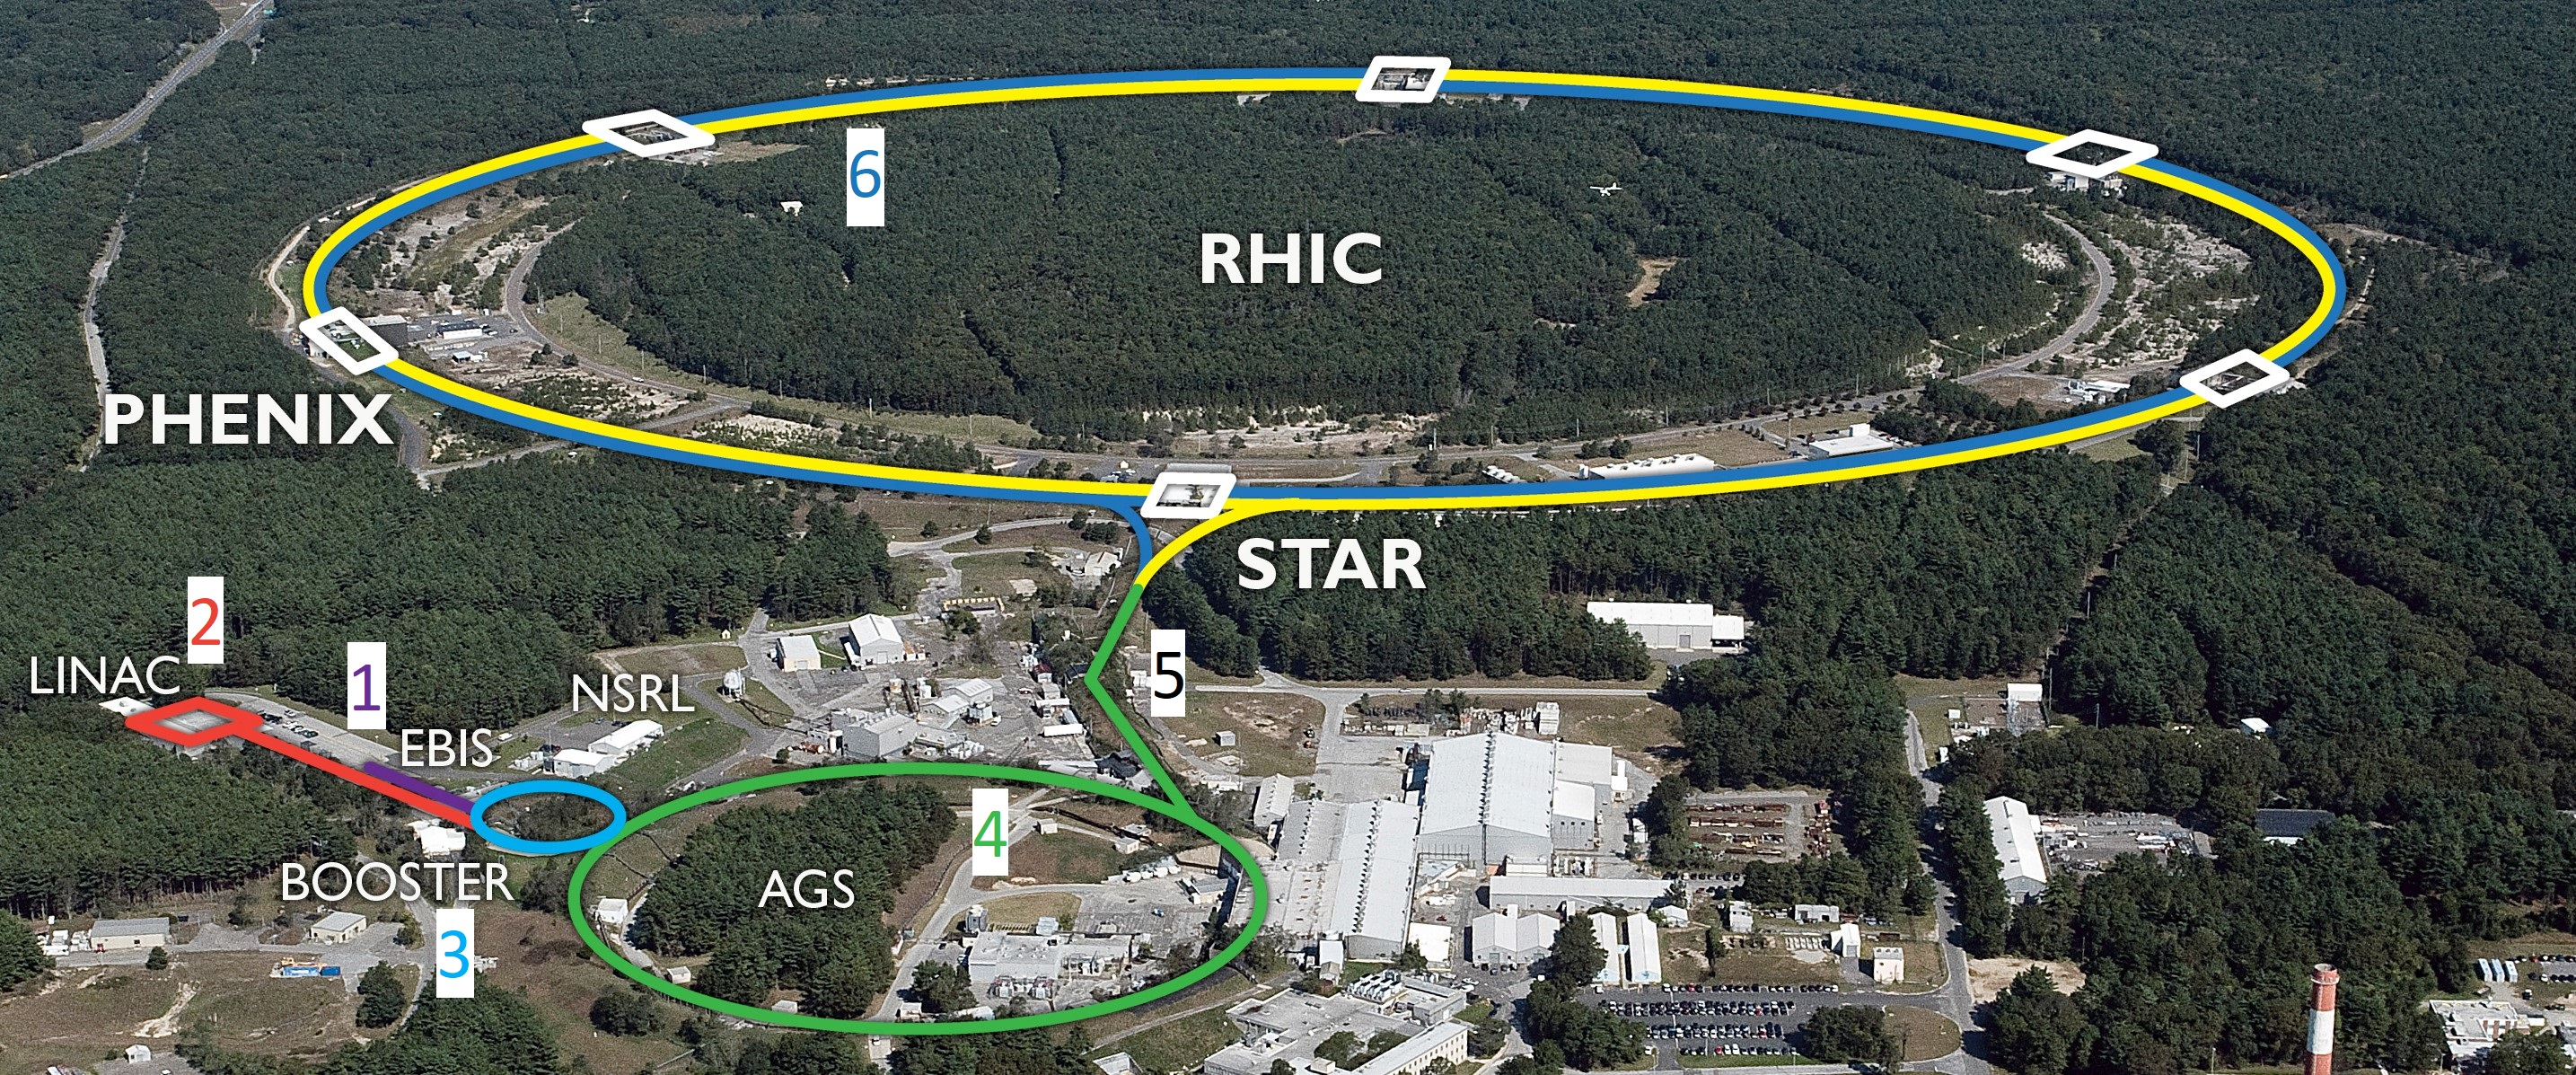
\includegraphics[scale=0.5]{images/written.jpg}
    \end{figure}
\end{frame}

\begin{frame}{Επιτάχυνση Ιόντων}
    \begin{figure}
        \centering
        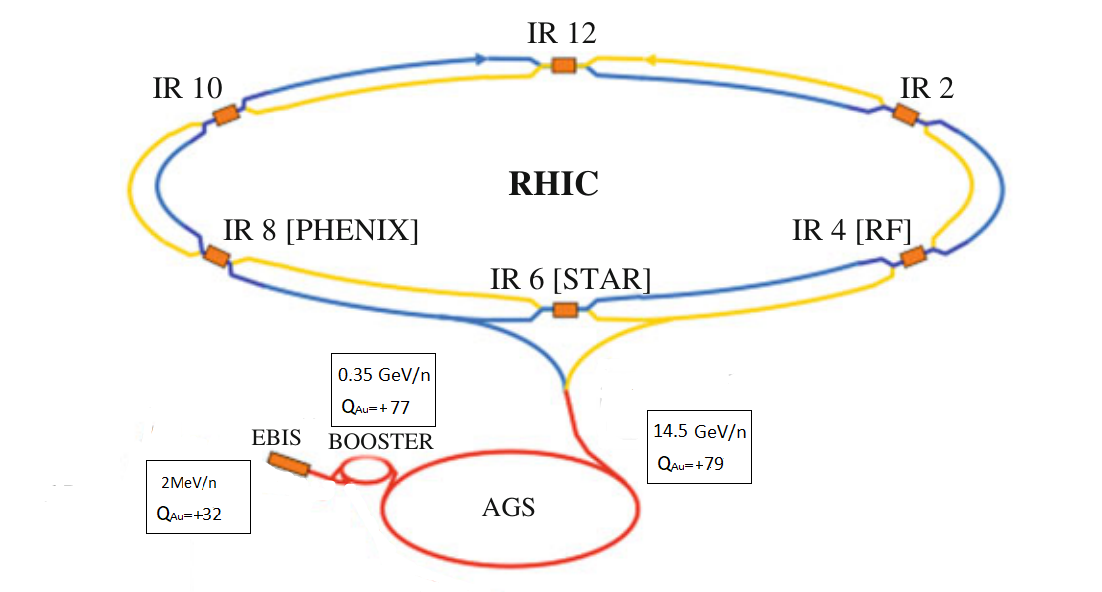
\includegraphics[scale=0.6]{images/RHIC_full_ions.png}
    \end{figure}

    \begin{table}[h!]
        \centering
        \begin{tabular}{c|cccc}
      Στάδιο   & Πηγή Ιόντων   &  Booster    & AGS       & RHIC\\
      Ενέργεια &  2MeV/n       & 0.35GeV/n   & 14.5GeV/n & 100GeV/n\\
      Φoρτίο Εξόδου  & +32           & +77         &  +79      & -
        \end{tabular}
    \end{table}
\end{frame}

\begin{frame}{Επιτάχυνση Πρωτονίων}
    \begin{figure}
        \centering
        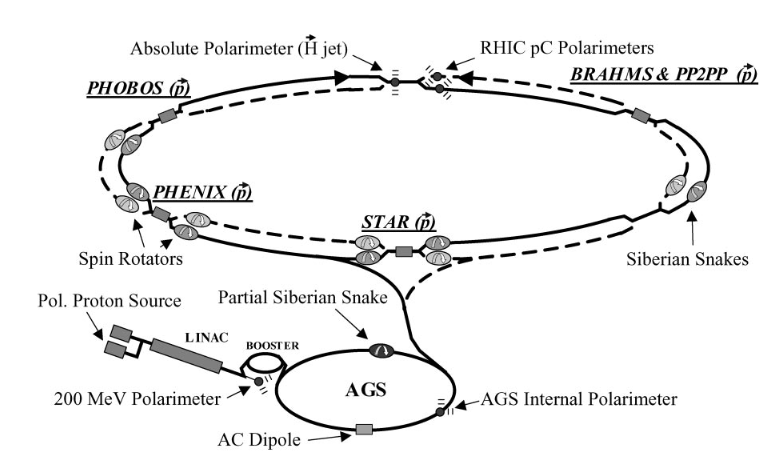
\includegraphics[scale=0.7]{images/protons_path.png}
    \end{figure}

\begin{table}[]
        \centering
        \begin{tabular}{c|cccc}
      Στάδιο         & Πηγή Ιόντων   &  LINAC    & AGS       & RHIC\\
      Ενέργεια       &  2MeV       &  2.4GeV   & 24.3GeV & 500GeV\\
      Πόλωση Εξόδου  & 80-85\%       &         &       & 50-60\%
        \end{tabular}
    \end{table}
\end{frame}
    
%--------------------------------------------------------------------------
%           END ACCELERATION
%--------------------------------------------------------------------------
%
%
%===================================================================
%           BEGIN DETECTOR SUBSYSTEMS 
%===================================================================
%
%
%-------------   TPC \begin{frame}{Frame Title}
   
\begin{frame}{Time Projection Chamber (TPC)}
     \begin{minipage}{0.4\textwidth}
        \begin{itemize}
            \item[$\star$] Μήκος $4.2m \&$ Ακτίνα 4m 
            \item[$\star$] Ανακατασκευή τροχιών φορτισμένων σωματιδίων ορμής $100MeV/c  -  10GeV/c$
            \item[$\star$] Μέτρηση ορμής φορτισμένων σωματιδίων ορμής $100MeV/c  - 30GeV/c$
            \item[$\star$]
        \end{itemize}
    \end{minipage}
    \begin{minipage}{0.55\textwidth}
        % column 2
        \begin{figure}
            \centering
            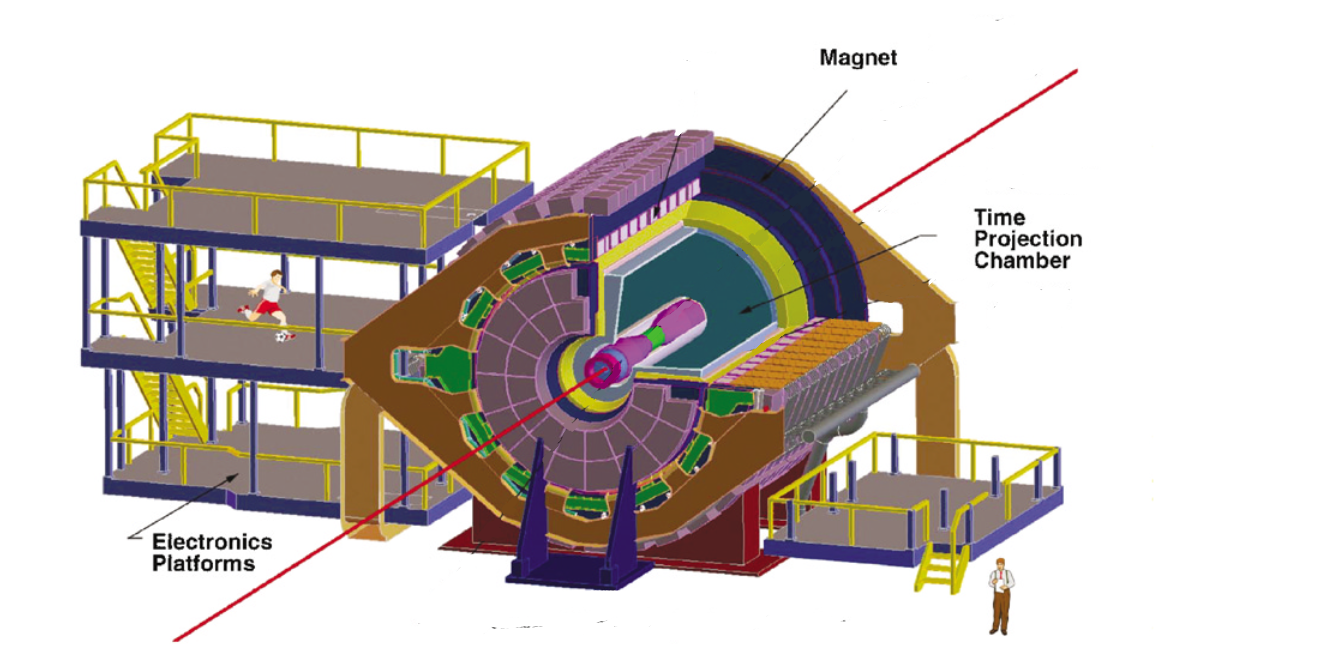
\includegraphics[scale=0.5]{images/Star_TPC_Magnets.png}]
        \end{figure}
    \end{minipage}
\end{frame}
%---------------------------
\begin{frame}{TPC - Γεωμετρικά Όρια}
    \begin{minipage}{0.55\textwidth}
        \begin{figure}
            \centering
            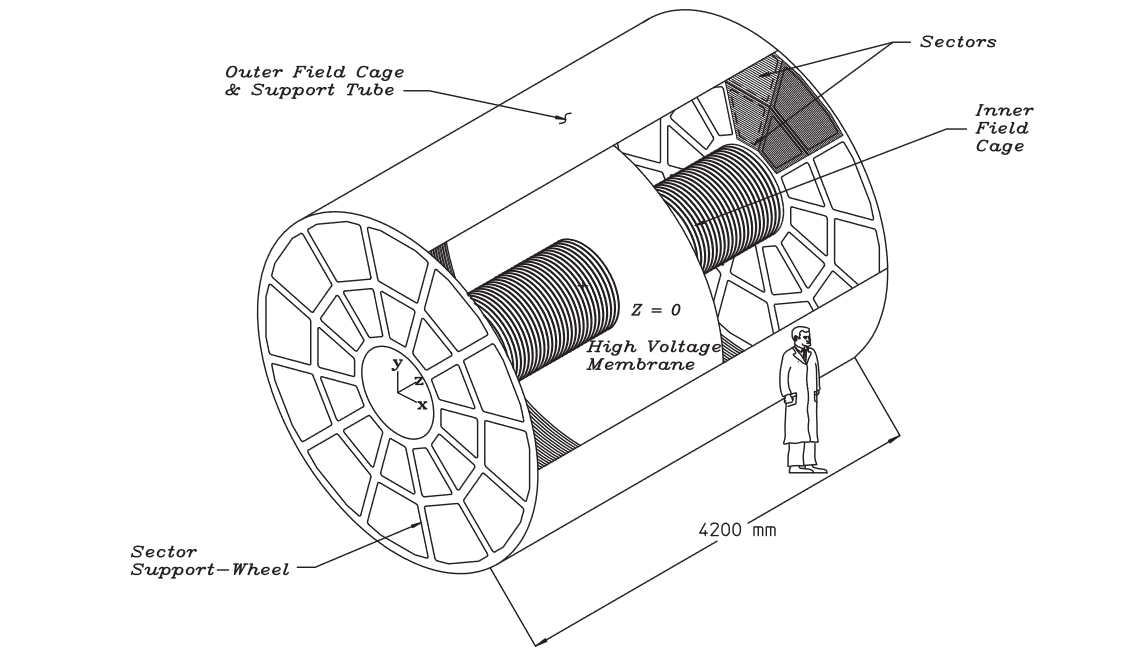
\includegraphics[scale=0.4]{images/TPC_sketch.png}
        \end{figure}
    \end{minipage}
     \begin{minipage}{0.4\textwidth}
        % column 1
        \begin{itemize}
            \item[$\star$] Γεωμένος Εσωτερικός \& Εξωτερικός Κύλινδρος \& Βάσεις σε Δυναμικό 0V
            \item[$\star$] Μεμβράνη στο Κέντρο του Κυλίνδρου σε δυνομικό 28kV
            \item[$\star$] Δημιουργία "Ομογενούς" Ηλεκτρικού Πεδίου για την ολίσθηση των δευτερογενών σωματιδίων προς τις βάσεις 
            \item[$\star$] Κατεύθυνση Πεδίου: Κεντρική Μεμβράνη $\rightarrow$  Βάσεις 
        \end{itemize}
    \end{minipage}
\end{frame}
%--------------------------
\begin{frame}{TPC Γεωμετρικά Όρια: End Caps}
    
        \begin{itemize}
            \item[$\star$] Αποτελείται από 12 όμοια μέρη 
            \item[$\star$] Δομική Μονάδα: MultiWire Proportional Chamber (MWPC)
            \item[$\star$] Δομή MWPC(βάση προς θάλαμος):
                \begin{itemize}
                      \item  Pads-Κάθοδοι \pause   %$\rightarrow$\\      
                      \item  Επίπεδο Συρμάτινων Ανόδων (Δημιουργία Διαφοράς Δυναμικού και λειτουργία στην Αναλογική Περιοχή) \pause%$\xrightarrow{}$\\
                      \item  Πλέγμα θωράκισης (Περιορισμός Αναλογικής Περιοχής) \pause%$\xrightarrow{}$ \\
                      \item  Gating Grid (Περιορισμός διαφυγής ιόντων \& "Φιλτράρισμα" σωματιδίων που εισέρχονται στην αναλογική περιοχή)\pause
                \end{itemize}
            \item[$\star$] Στο κάθε μέρος υπάρχει διαφορετική διαρρύθμιση των pads
            \item[$\star$] \textit{Εξωτερικό:} Πυκνότερα pads για αύξηση της διακριτικής ικανότητας $dE/dx$ και διάκρισης σωματιδίων και ανακατασκευή τροχιάς
            \item[$\star$] \textit{Εσωτερικό:} Αραιότερα pads διότι λόγω αυξημένης πυκνότητας θέλουμε μόνο τον διάκριση μεταξύ δύο τροχιών
        \end{itemize}
    
\end{frame}
%------------------------------
\begin{frame}{TPC}
   \begin{figure}[h!]
    \centering
    \begin{minipage}{.5\textwidth}
        \centering
        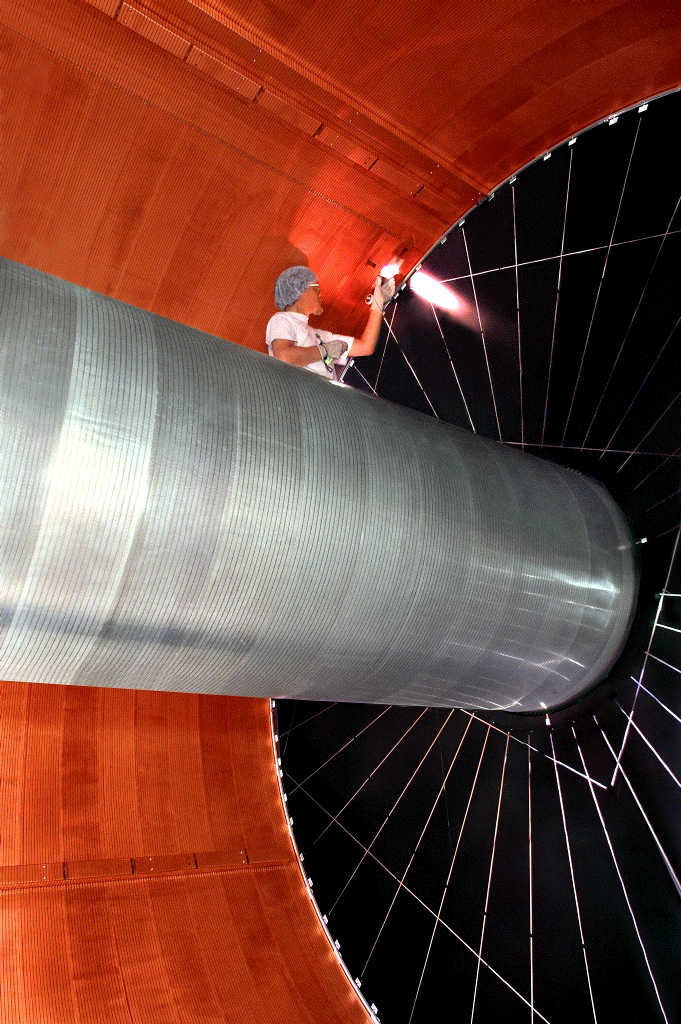
\includegraphics[scale=0.25]{images/TPC_inside.jpg}
    \end{minipage}%
    \begin{minipage}{0.5\textwidth}
        \centering
        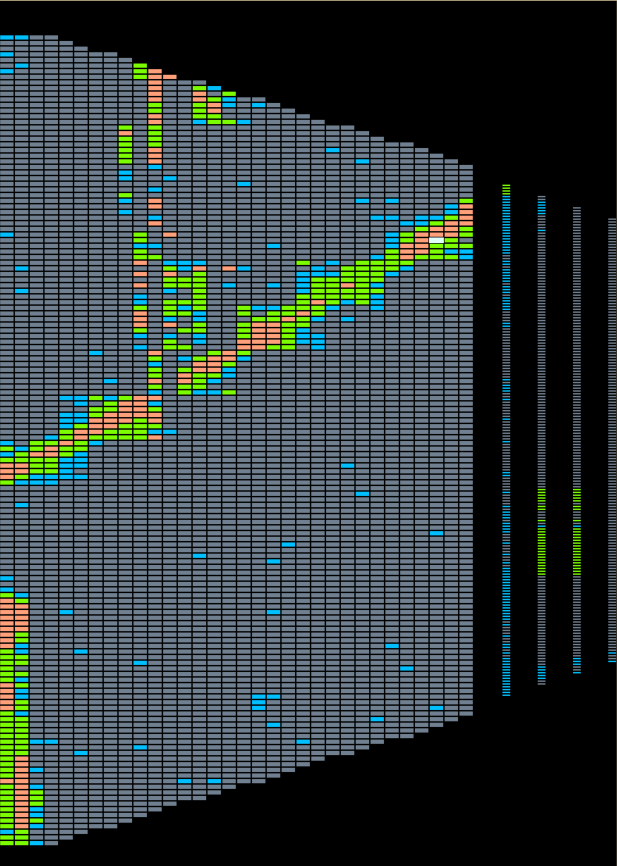
\includegraphics[scale=0.45]{images/TPC_endcap_traj.png}   
    \end{minipage}
\end{figure}		 	
		 	
\end{frame}
%--------------------------------
\begin{frame}{TPC - Mίγμα Αερίων}
    \begin{minipage}{0.55\textwidth}
        % column 2
        \begin{figure}
            \centering
            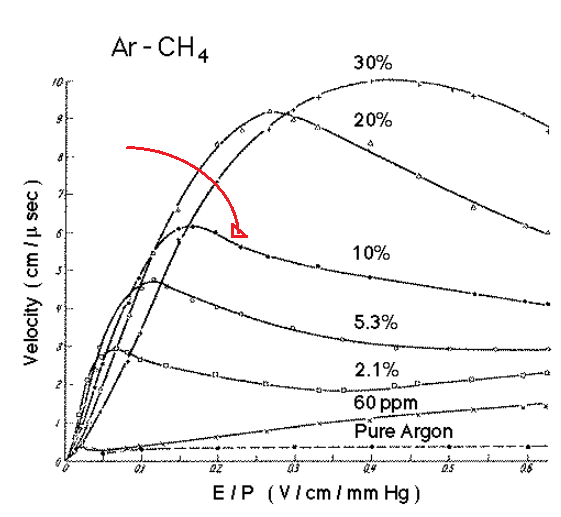
\includegraphics[scale=0.6]{images/TPC_gases.png}
        \end{figure}
    \end{minipage}
         \begin{minipage}{0.4\textwidth}
        % column 1
        \begin{itemize}
            \item[$\star$] 50.000lt  από 10\% $CH_4$ - 90\% Ar 
            \item[$\star$] Κριτήρια: Καθαρότητα \& Ευκολία στην Διατήρησή της, ταχύτητα ολίσθησης, ασφάλεια, κόστος
            \item[$\star$] Μείωση Ηλεκτραρνητικών Στοιχείων $\rightarrow$ $O_2<100ppm$ \& $H_2O<10ppm$ 
            \item[$\star$] Eπιλογή πεδίου ώστε η ταχύτητα ολίσθησης να μην είναι στο μέγιστο της καμπύλης
        \end{itemize}
    \end{minipage}
\end{frame}
%------------------------------
\begin{frame}{Επίδοση}
     \begin{minipage}{0.47\textwidth}
        \begin{figure}
            \centering
            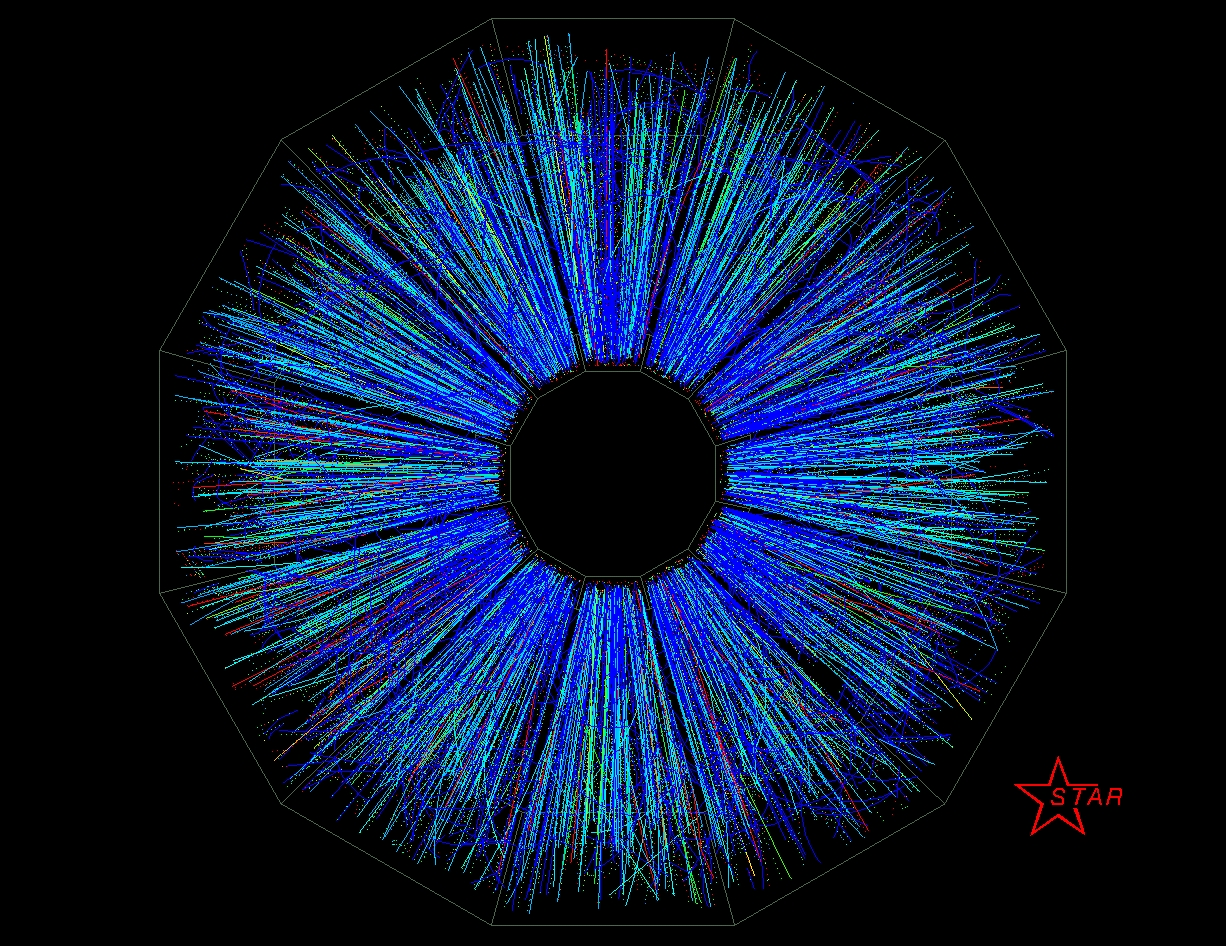
\includegraphics[scale=0.15]{images/TPC_recon.png}
        \end{figure}
        \begin{figure}
            \centering
            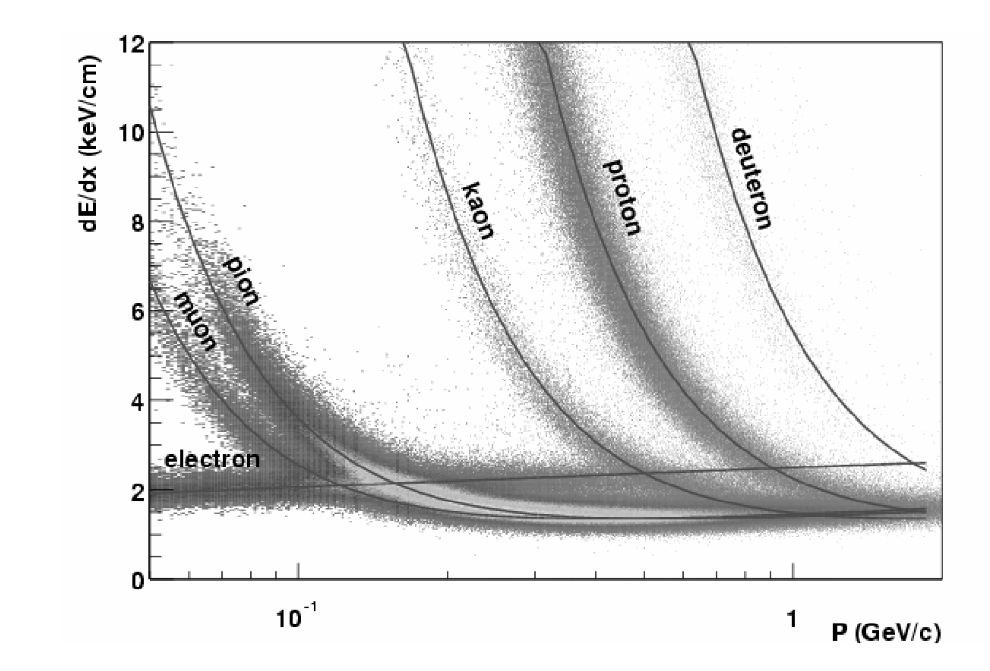
\includegraphics[scale=0.35]{images/TPC_ident.png}
        \end{figure}
    \end{minipage}
    \begin{minipage}{0.5\textwidth}
        \begin{itemize}
            \item[$\star$] Περίπου το 30\% των τροχιών των δευτερογενών σωματιδίων επικαλύπτεται
            \item[$\star$] Σε όσες επικαλύπτονται χρησιμοποιούνται αλγόριθμοι για την για τον διαχωρισμό τους, ενώ ο προσδιορισμός του dE/dx είναι εφικτός
            \item[$\star$] Προσδιορισμός της θέσης στο επίπεδο της τροχιάς από τα pads που δίνουν σήμα
            \item[$\star$] Προσδιορισμός της θέσης κάθετα στο επίπεδο των end caps από τον χρόνο πτήσης
         \end{itemize}
    \end{minipage}
\end{frame}

%
%-----------------------------------
%------------ FTPC
%------------------------------------
%
%

\begin{frame}{Forward Time Projection Chamber (FTPC)}
     \begin{minipage}{0.4\textwidth}
        % column 1 
        \begin{itemize}
            \item[$\star$] Δύο κυλινδρικοί TPC με αέριο σε ακτίνα $7.7cm<R_{FTCP}<30.05cm$ και μήκος 1.2m
            \item[$\star$] Καλύπτουν μεγάλες pseudorapidity $2.5<|\eta|<4.0$
            \item[$\star$] Ίδια αρχή λειτουργίας με τον TPC 
        \end{itemize}
    \end{minipage}
    \begin{minipage}{0.5\textwidth}
        % column 2
      
        \begin{figure}
            \centering
            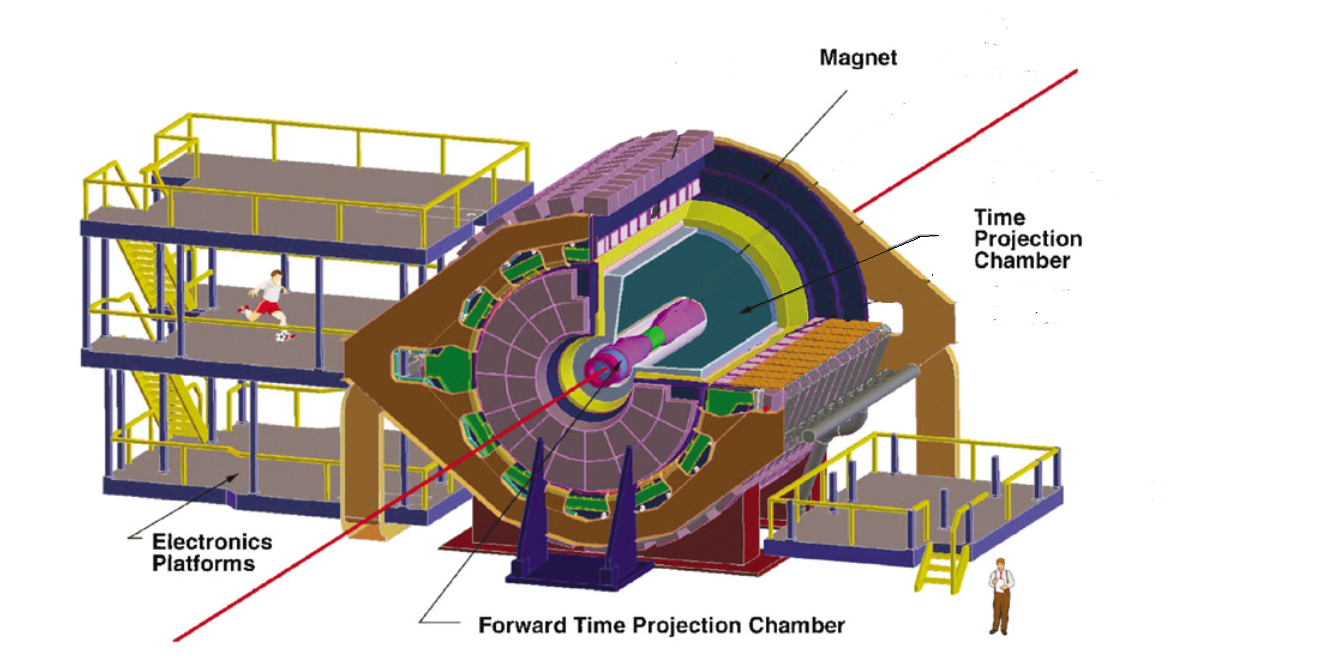
\includegraphics[scale=0.5]{images/Star_FTPC.png}
        \end{figure}
    \end{minipage}
\end{frame}
%-------------------------------------------


\begin{frame}{FTPC}
     \begin{minipage}{0.47\textwidth}
        % column 
        \begin{itemize}
            \item[$\star$] \textcolor{red}{Διαφορά} από TPC
                \begin{itemize}
                    \item Το πεδίο είναι ακτινικό
                    \item Άρα η ολίσθηση των δευτερογενών σωματιδίων είναι ακτινική 
                    \item Οι MWPC είναι στον εξωτερικό φλοιό και τα pads σε καμπύλο σχήμα
                \end{itemize}
          %  \item[$\star$] Ανακατασκευή Τροχιών
          %      \begin{itemize}
          %          \item Ανίχνευση Θέσεων στα pads που δίνουν σήμα
          %          \item Ομαδοποίηση των σημάτων
          %      \end{itemize}
        \end{itemize}
    \end{minipage}
    \begin{minipage}{0.5\textwidth}
        % column 2
        \begin{figure}
            \centering
            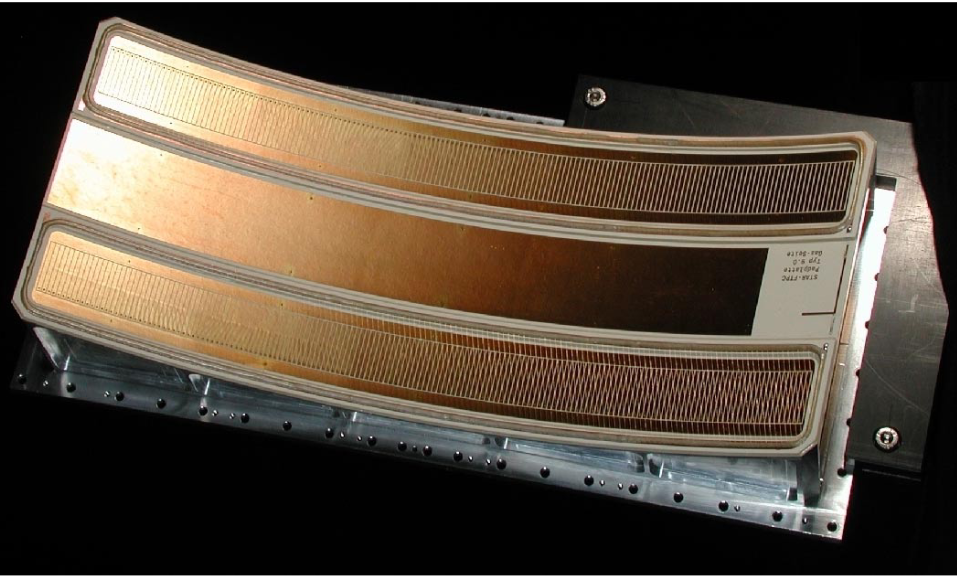
\includegraphics[scale=0.3]{images/FTPC.png}
        \end{figure}
        \begin{figure}
            \centering
            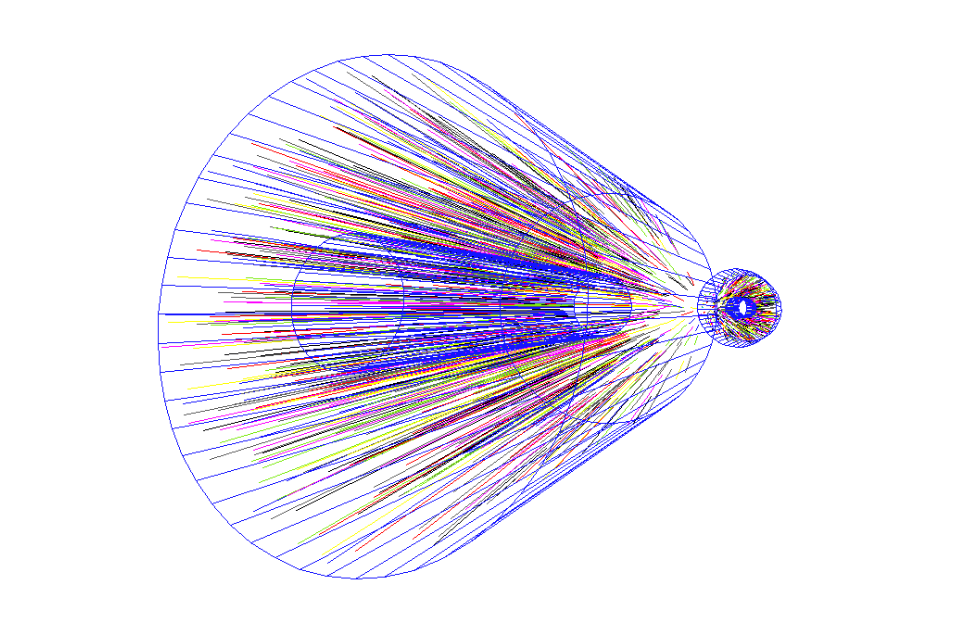
\includegraphics[scale=0.3]{images/FTPC_reconstruction.png}
        \end{figure}
    \end{minipage}
\end{frame}




%----------- BEMC 
\begin{frame}{Barrel Electromagnetic Calorimeter (BEMC)}
     \begin{minipage}{0.47\textwidth}
        % column 1
        \begin{itemize}
            \item[$\star$] Για κάλυψη pseudorapidity $|\eta|<1$ με συνολική επιφάνεια $60m^2$ για σωματίδια με υψηλή ορμή
            \item[$\star$] Είναι τοποθετημένο εντός του μαγνητικού πεδίου του σωληνοειδούς
            \item[$\star$] Αποτελείται από διακριτά κομμάτια Scintillating Sampling Calorimeters με Μόλυβδο
        \end{itemize}
    \end{minipage}
    \begin{minipage}{0.5\textwidth}
        % column 2
        \begin{figure}
            \centering
            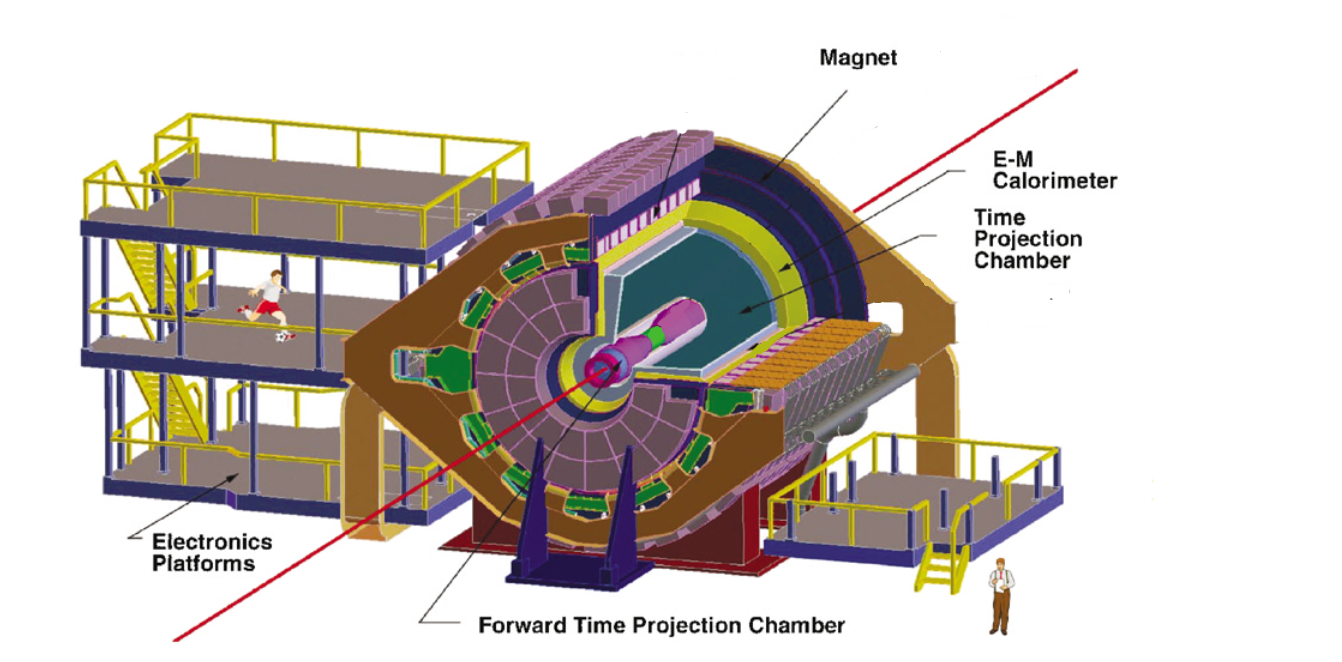
\includegraphics[scale=0.5]{images/Star__BEMC.png}
        \end{figure}
    \end{minipage}
\end{frame}

\begin{frame}{BEMC}
    \begin{minipage}{0.47\textwidth}
        % column 1
        \begin{figure}
            \centering
            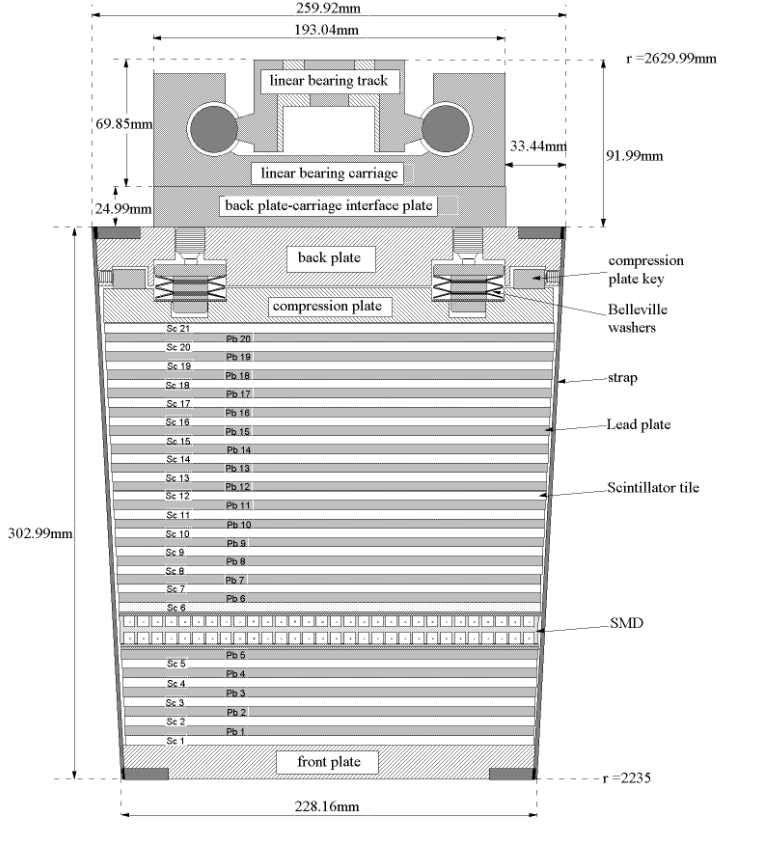
\includegraphics[scale=0.3]{images/BEMC_side_view2.png}
        \end{figure}
    \begin{figure}
        \centering
        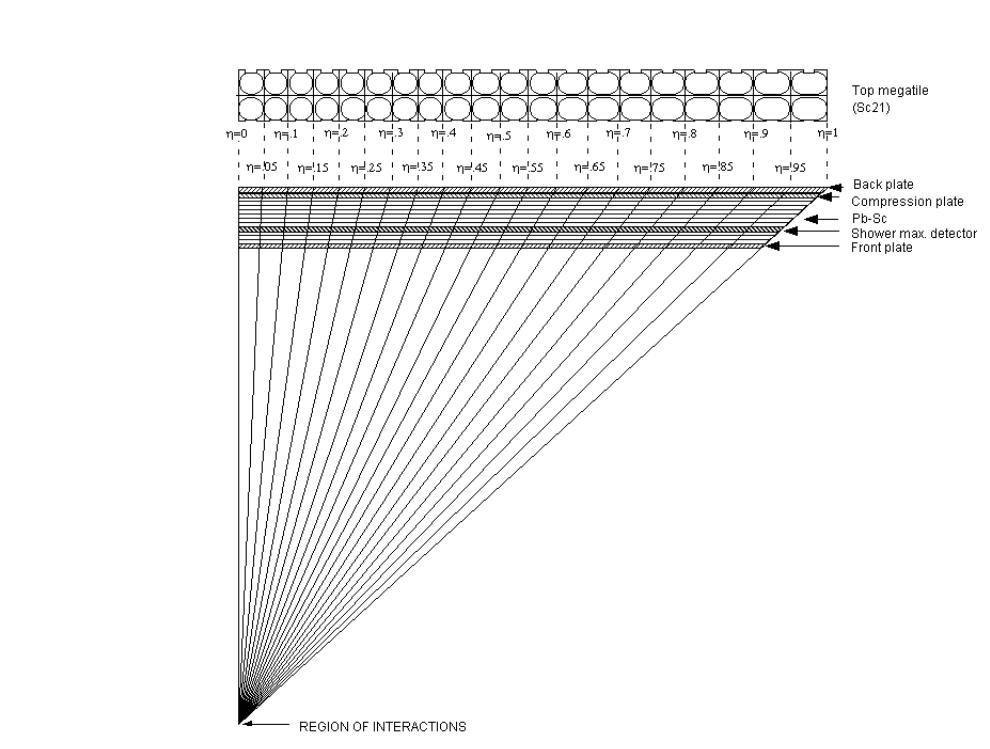
\includegraphics[scale=0.3]{images/BEMC_side_view.png}
    \end{figure}
    \end{minipage}
    \begin{minipage}{0.5\textwidth}
        % column 2
        \begin{itemize}
            \item[$\star$] Το κάθε τμήμα σπινθηριστή συνδέεται με τους φωτοπολλαπλασιαστές μέσω μίας οπτικής ίνας
            \item[$\star$] Oι φωτοπολλαπλασιαστές είναι εκτός του χώρου με το μαγνητικό πεδίο, λόγω έλλειψης χώρου άρα λειτουργούν και σε μηδενικό μαγνητικό πεδίο χωρίς να πρέπει να τους προφυλλάξουμε με επιπλέον υλικό
            \item[$\star$] Σε βάθος 5.6$X_0$ από την αρχή των στρωμάτων έχουμε το μέγιστο της ενέργειας καταιγισμού
            \item[$\star$] Εκεί υπάρχει ένας αναλογικός ανιχνευτής αερίου ο οποίος βοηθά στην ταυτοποίηση των $\pi^0,\gamma,e$
        \end{itemize}
    \end{minipage}
\end{frame}

%
%
%------------ SSD 
%


%
%----------------------------------------------------------------------
%           END DETECTORS 
%---------------------------------------------------------------------
%
%
%======================================================================
%           START RESULTS 
%=====================================================================
% 
% 
% 
\begin{frame}{Συγκρούσεις Βαρέων Ιόντων}{Θεωρητικά}
    \begin{itemize}
        \item[$\star$] \underline{$\tau<0$:} Πριν την σύγκρουση όπου Κουάρκ και Γλουόνια υπάρχουν στα νουκλεόνια του πυρήνα 
         \item[$\star$] \underline{$0<\tau<\tau_0$:} Η αρχική κινητική ενέργεια εναποτίθεται στην περιοχή επικάλυψης των πυρήνων φτιάχνοντας μία κατάσταση που καλείται fireball.
         
         Αν η αρχική ενέργεια είναι αρκετά μεγάλη δημιουργείται μία κατάσταση στην οποία τα κουάρκ και τα γλουόνια αποδεσμεύονται από τα νουκλεόνια και φτιάχνουν το Quark Gluon Plasma (QGP) \pause
          \item[$\star$] \underline{$\tau_0<\tau<\tau_f$:} Οι συνεχείς συγκρούσεις μεταξύ των συστατικών της fireball οδηγούν το σύστημα με θερμική ισορροπία και σε διαστολή.

          Όσο το σύστημα διαστέλλεται ταυτόχρονα κρυώνει μέχρι να φτάσει σε μία κρίσιμη θερμοκρασία \textbf{$T_c$} κάτω από την οποία αρχίζει η \textit{αδρονοποίηση} , δηλαδή η επαναδημιουργία νέων αδρονίων που δεν είναι αποκλειστικά νετρόνια και πρωτόνια. \pause
           \item[$\star$] \underline{$\tau>\tau_f$:} Εδώ επέρχεται και η λεγόμενη \textit{χημική ισορροπία}, οι ανελαστικές συγκρούσεις παύουν (\textit{chemical freeze-out}) και καθώς η θερμοκρασία συνεχίζει να μειώνεται η μέση ελεύθερη διαδρομή γίνεται μεγαλύτερη από τις διαστάσεις του συστήματος και σταματούν οι ελαστικές συγκρούσεις (\textit{kinetic freeze-out}). \pause
            \item[\textcolor{red}{$\rightarrow$}] Η μετάβαση φάσης αναμένεται θεωρητικά να συμβαίνει σε θερμοκρασία $170MeV \rightarrow 2TK$
    \end{itemize}
\end{frame}

\begin{frame}{Συγκρούσεις Βαρέων Ιόντων}{Θεωρητικά}
    \begin{figure}
        \centering
        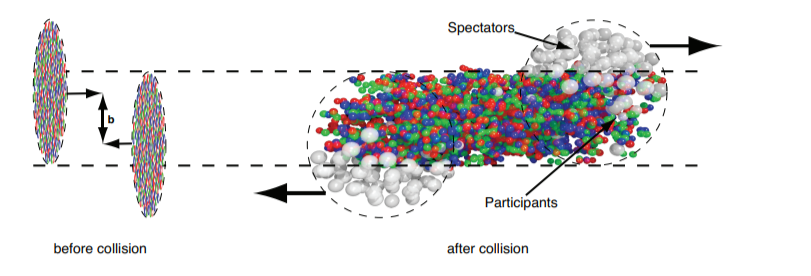
\includegraphics{images/ion_collisions.png}
    \end{figure}
\end{frame}

%\begin{frame}{Συγκρούσεις Βαρέων Ιόντων}{Θεωρητικά}
%    \begin{figure}
%        \centering
%        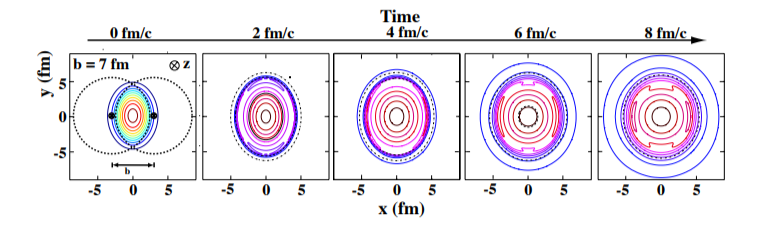
\includegraphics{images/ion_collisions_noncentral.png}
%    \end{figure}
%\end{frame}

\begin{frame}{Συγκρούσεις Βαρέων Ιόντων}{Θεωρητικά}
    \begin{figure}
        \centering
        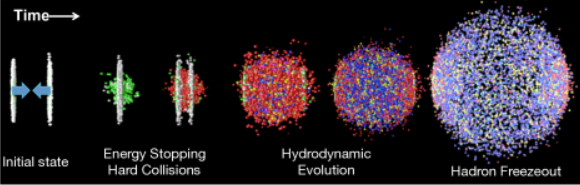
\includegraphics[scale=1.2]{images/QGP_formation2.png}
    \end{figure}
\end{frame}

\begin{frame}{Συγκρούσεις Βαρέων Ιόντων}{Πειραματικά, soft range $p_T<1.5GeV/c$}
    \begin{minipage}{0.47\textwidth}
        % column 1
        \begin{figure}
            \centering
            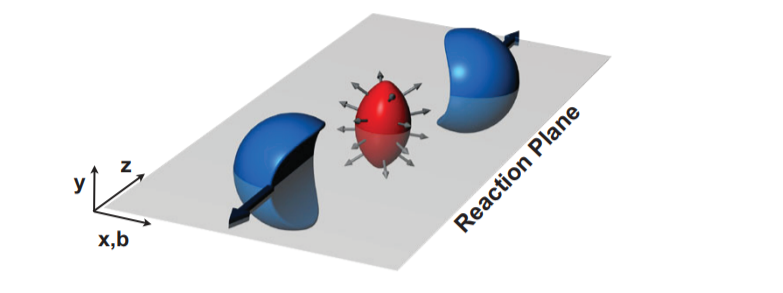
\includegraphics[scale=0.5]{images/ion_collisions_elliptic.png}
        \end{figure}
    \end{minipage}
    \begin{minipage}{0.5\textwidth}
        % column 2
        \begin{itemize}
            \item[$\star$] Θεωρητικές ενδείξεις πως η ροή σωματιδίων με μικρές ορμές δεν είναι ισοτροπική. 

            Ποσοτικοποίηση μέσω του συντελεστή \textit{elliptical flow}, $v_2$

            \item[$\star$] Παρατηρήθηκε πως η ροή είναι συλλογκή και ανισοτροπική με διαφορετικό τρόπο για κάθε είδος παραγόμενων σωματιδίων
        \end{itemize}
    \end{minipage}
\end{frame}

\begin{frame}{Συγκρούσεις Βαρέων Ιόντων}{Πειραματικά, soft range $p_T<1.5GeV/c$}
    \begin{figure}
        \centering
        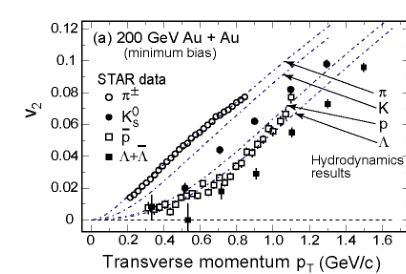
\includegraphics[scale=1.2]{images/result_soft_1.png}
    \end{figure}
\end{frame}

\begin{frame}{Συγκρούσεις Βαρέων Ιόντων}{Jet Quenching}
    \begin{itemize}
        \item[$\star$] Oι συγκρούσεις των παρτονίων οδηγούν σε κουάρκ και γλουόνια μεγαλύτερων ορμών δημιουργούν δύο αντιδιαμετρικά jets σε αρχικά στάδια της σύγκρουσης, πριν την δημιουργία του QGP
        \item[$\star$] Αν τα jets δημιουργηθούν ακριβώς πριν  το QGP, τότε το ένα θα διέλθει μεσα απ' το QGP.
        Αυτό, ενδέχεται να χάσει αρκετή ενέργεια ώστε να μην μπορέσουν να δημιουργηθούν τα ανιχνεύσιμα αδρόνια \pause
    \end{itemize}
    \begin{figure}
        \centering
        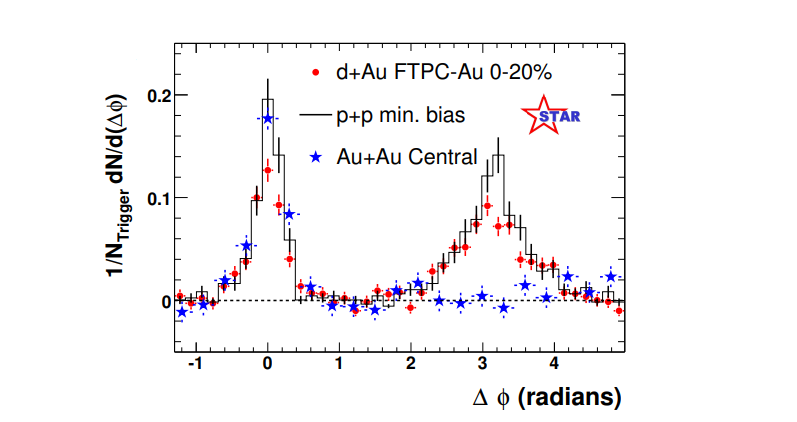
\includegraphics[scale=0.7]{images/jet_quenching.png}
    \end{figure}
\end{frame}



\begin{frame}{Συγκρούσεις Βαρέων Ιόντων}{Παραγωγή (Anti)-Hypertriton}
      \begin{table}[h!]
    \centering
    \begin{tabular}{cc}
       $^3_{\Lambda}H$ :  p-n-$\Lambda$ & $^3_{\bar{\Lambda}}\bar{H}$ :  $\bar{p}-\bar{n}-\bar{\Lambda}$
    \end{tabular}
\end{table}
    \begin{itemize}
        \item[$\star$] Οι παραπάνω πυρήνες είναι εξαιρετικά αστθείς 
        \item[$\star$] Ανιχνεύονται τα παράγωγα των διασπάσεών τους , π.χ. $^3_{\bar{\Lambda}}\bar{H}\rightarrow\bar{He} + \pi^+$\pause
    \end{itemize}

     
        % column 2
        \begin{figure}
            \centering
            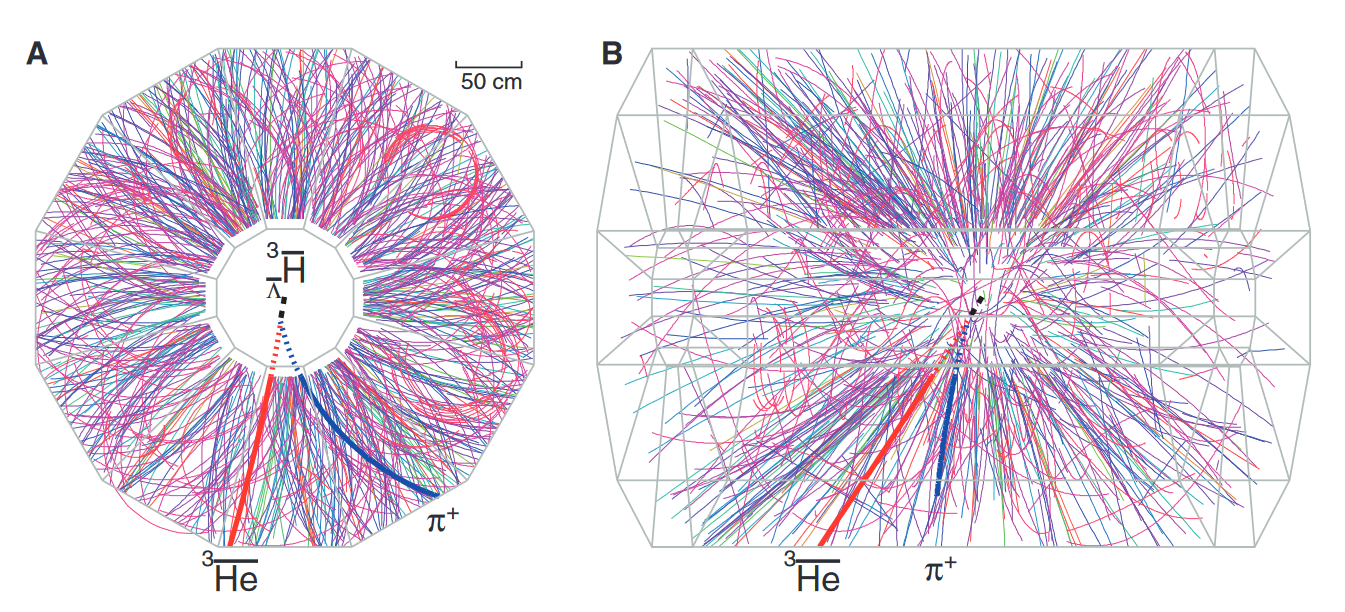
\includegraphics[scale=0.4]{images/hypertriton_traj.png}
        \end{figure}
\end{frame}

\begin{frame}{Συγκρούσεις Βαρέων Ιόντων}{Παραγωγή (Anti)-Hypertriton}
            \begin{itemize}
                \item[$\star$] Μέτρηση μάζας πυρήνα - αντιπυρήνα \& συμφωνία στα όρια του σφάλματος (αναμενόμενο)
                    \begin{itemize}
                        \item  $m(^3_{\Lambda}H) = 2.989\pm0.001\pm0.002GeV/c^2$
                        \item  $m(^3_{\bar{\Lambda}}\bar{H}) = 2.991\pm0.001\pm0.002GeV/c^2$
                    \end{itemize}
                \item[$\star$] Μέτρηση χρόνου ζωής $\tau=182\pm27ps$ σε συμφωνία για τους δύο πυρήνες 
                \item[$\star$] Θεωρώντας πως η Ενέργεια Σύνδεσης είναι ίδια για τους δύο πυρήνες $B_\Lambda =0.41\pm0.12\pm0.11 MeV$
            \end{itemize}
        
        \end{frame}

\begin{frame}{Συγκρούσεις Βαρέων Ιόντων}{Παραγωγή (Anti)-Hypertriton}
    \begin{figure}
        \centering
        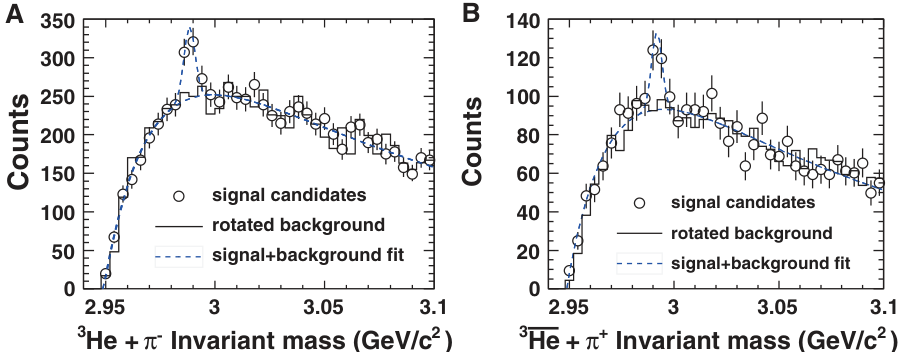
\includegraphics[scale=0.8]{images/hypertriton_mass.png}
    \end{figure}
\end{frame}










\end{document}